\chapter{Image recognition for IBD reconstruction with the SPMT system}
\label{sec:jcnn}

As explained in chapter \ref{sec:juno}, JUNO is an experiment composed of two systems, the Large Photo Tube Multiplier (LPMT) and the Small Photo Multiplier Tubes (SPMT). Both of the system observe the same physics event inside of the same medium but they differ in their photo-coverage, respectively 75.2\% and 2.7\%, their dynamic range, a thousands versus a few dozen, and their back-end electronics (see section \ref{sec:juno:LPMT}).

Due to their differences they are complementary and their strength and weakness. One important point the difference in expected resolution, the LPMT system outperform largely the SPMT system but is subject to effects such as saturation \cite{juno_collaboration_calibration_2021} that could bias the reconstruction, effect that the SPMT system is impervious to. Also, due to the dynamic range of the LPMT, in case of high energy and high density event such as core-collapse supernova, the LPMT system could saturate and the lack of photo-coverage become a benefit.

Thus it is important to have reconstruction and analysis combined but also dedicated to each system, taking into account the specificity. The subject of this work is to propose a machine learning algorithm for the SPMT reconstruction based on Convolutional Neural Network (CNN).

\section{Motivations}

% -------------- Plan for motivation section ----------------
\begin{itemize}
  \item Promise of machine learning -> Exploit raw data
  \item Victor already done reco for SPMT
  \item Can CNN give similar results ? Better results ?
  \item Multiple reco methods good for reconstruction
  \item Comparison, difference in behavior
\end{itemize}

As explained in chapter \ref{sec:ml}, Machine Learning (ML) algorithms shine when modeling complex distribution from a given dataset. In our case, we have access to complete monte-carlo simulation of our detector to produce arbitrary large datasets that could represent multiple years of data taking. Also, due to the nature of monte-carlo simulation we have access to exact truth of the modelled event like the position, energy and nature of the particle.

One of expectation when using data-driven, and so, machine learning algorithm is that the algorithm will be able to use the entirety of the raw information, preventing any loss in precision due to miss-modeling or simplification of the underlying physic process.


Another algorithm was developed in the collaboration for energy and vertex reconstruction \cite{lebrin_towards_2022} and will serve as a performance reference in this work. The two methods will also be studied event by event to try to understand and unveil coherence or incoherence between their performances.


\section{Method and model}
% --------------- Plan for method and model -----------------
\begin{itemize}
  \item JUNO is an array of sensor following a quasi uniform and istropic geometric repartition -> Basically pixels -> Image
  \item CNN is gud for image processing (cite a lot of things)
  \item Details the architecture (Inspired from VGG 16)
    \begin{itemize}
      \item Convolutional layers
      \item Pooling layers -> Twice the channels when pooling by 2 -> Keep the same "amount" of information
      \item Dropout (introduce overtraining, maybe introduce overfitting in ML chapter ?)
      \item Vectorization fed to FCDNN
    \end{itemize}
\end{itemize}

One of simplest way to look at JUNO data is to consider the detector as an array of geometrically distributed sensors on a sphere. Their repartition is almost homogeneous, on this sphere surface providing an almost equal amount of information per unit surface on this sphere. One kind of data representation that is ordered, presenting the same property as a plane is the image, which is a bounded discrete euclidian plane.

Using this representation we can arrange the SPMTs on this plane while keeping most of the neighbouring informations. The pros and cons of this representation is detailed in section \ref{sec:jcnn:data}.

The most common approach in machine learning for image processing and image recognition is the Convolutional Neural Network (CNN). It is widely used in research and industry \cite{simonyan_very_2015, ciresan_multi-column_2012, abbasi_convolutional_2021, maksimovic_cnns_2021} due to its strengths (see section \ref{ml:cnn}) and has proven its relevance in image processing.

\begin{figure}[ht]
  \centering
  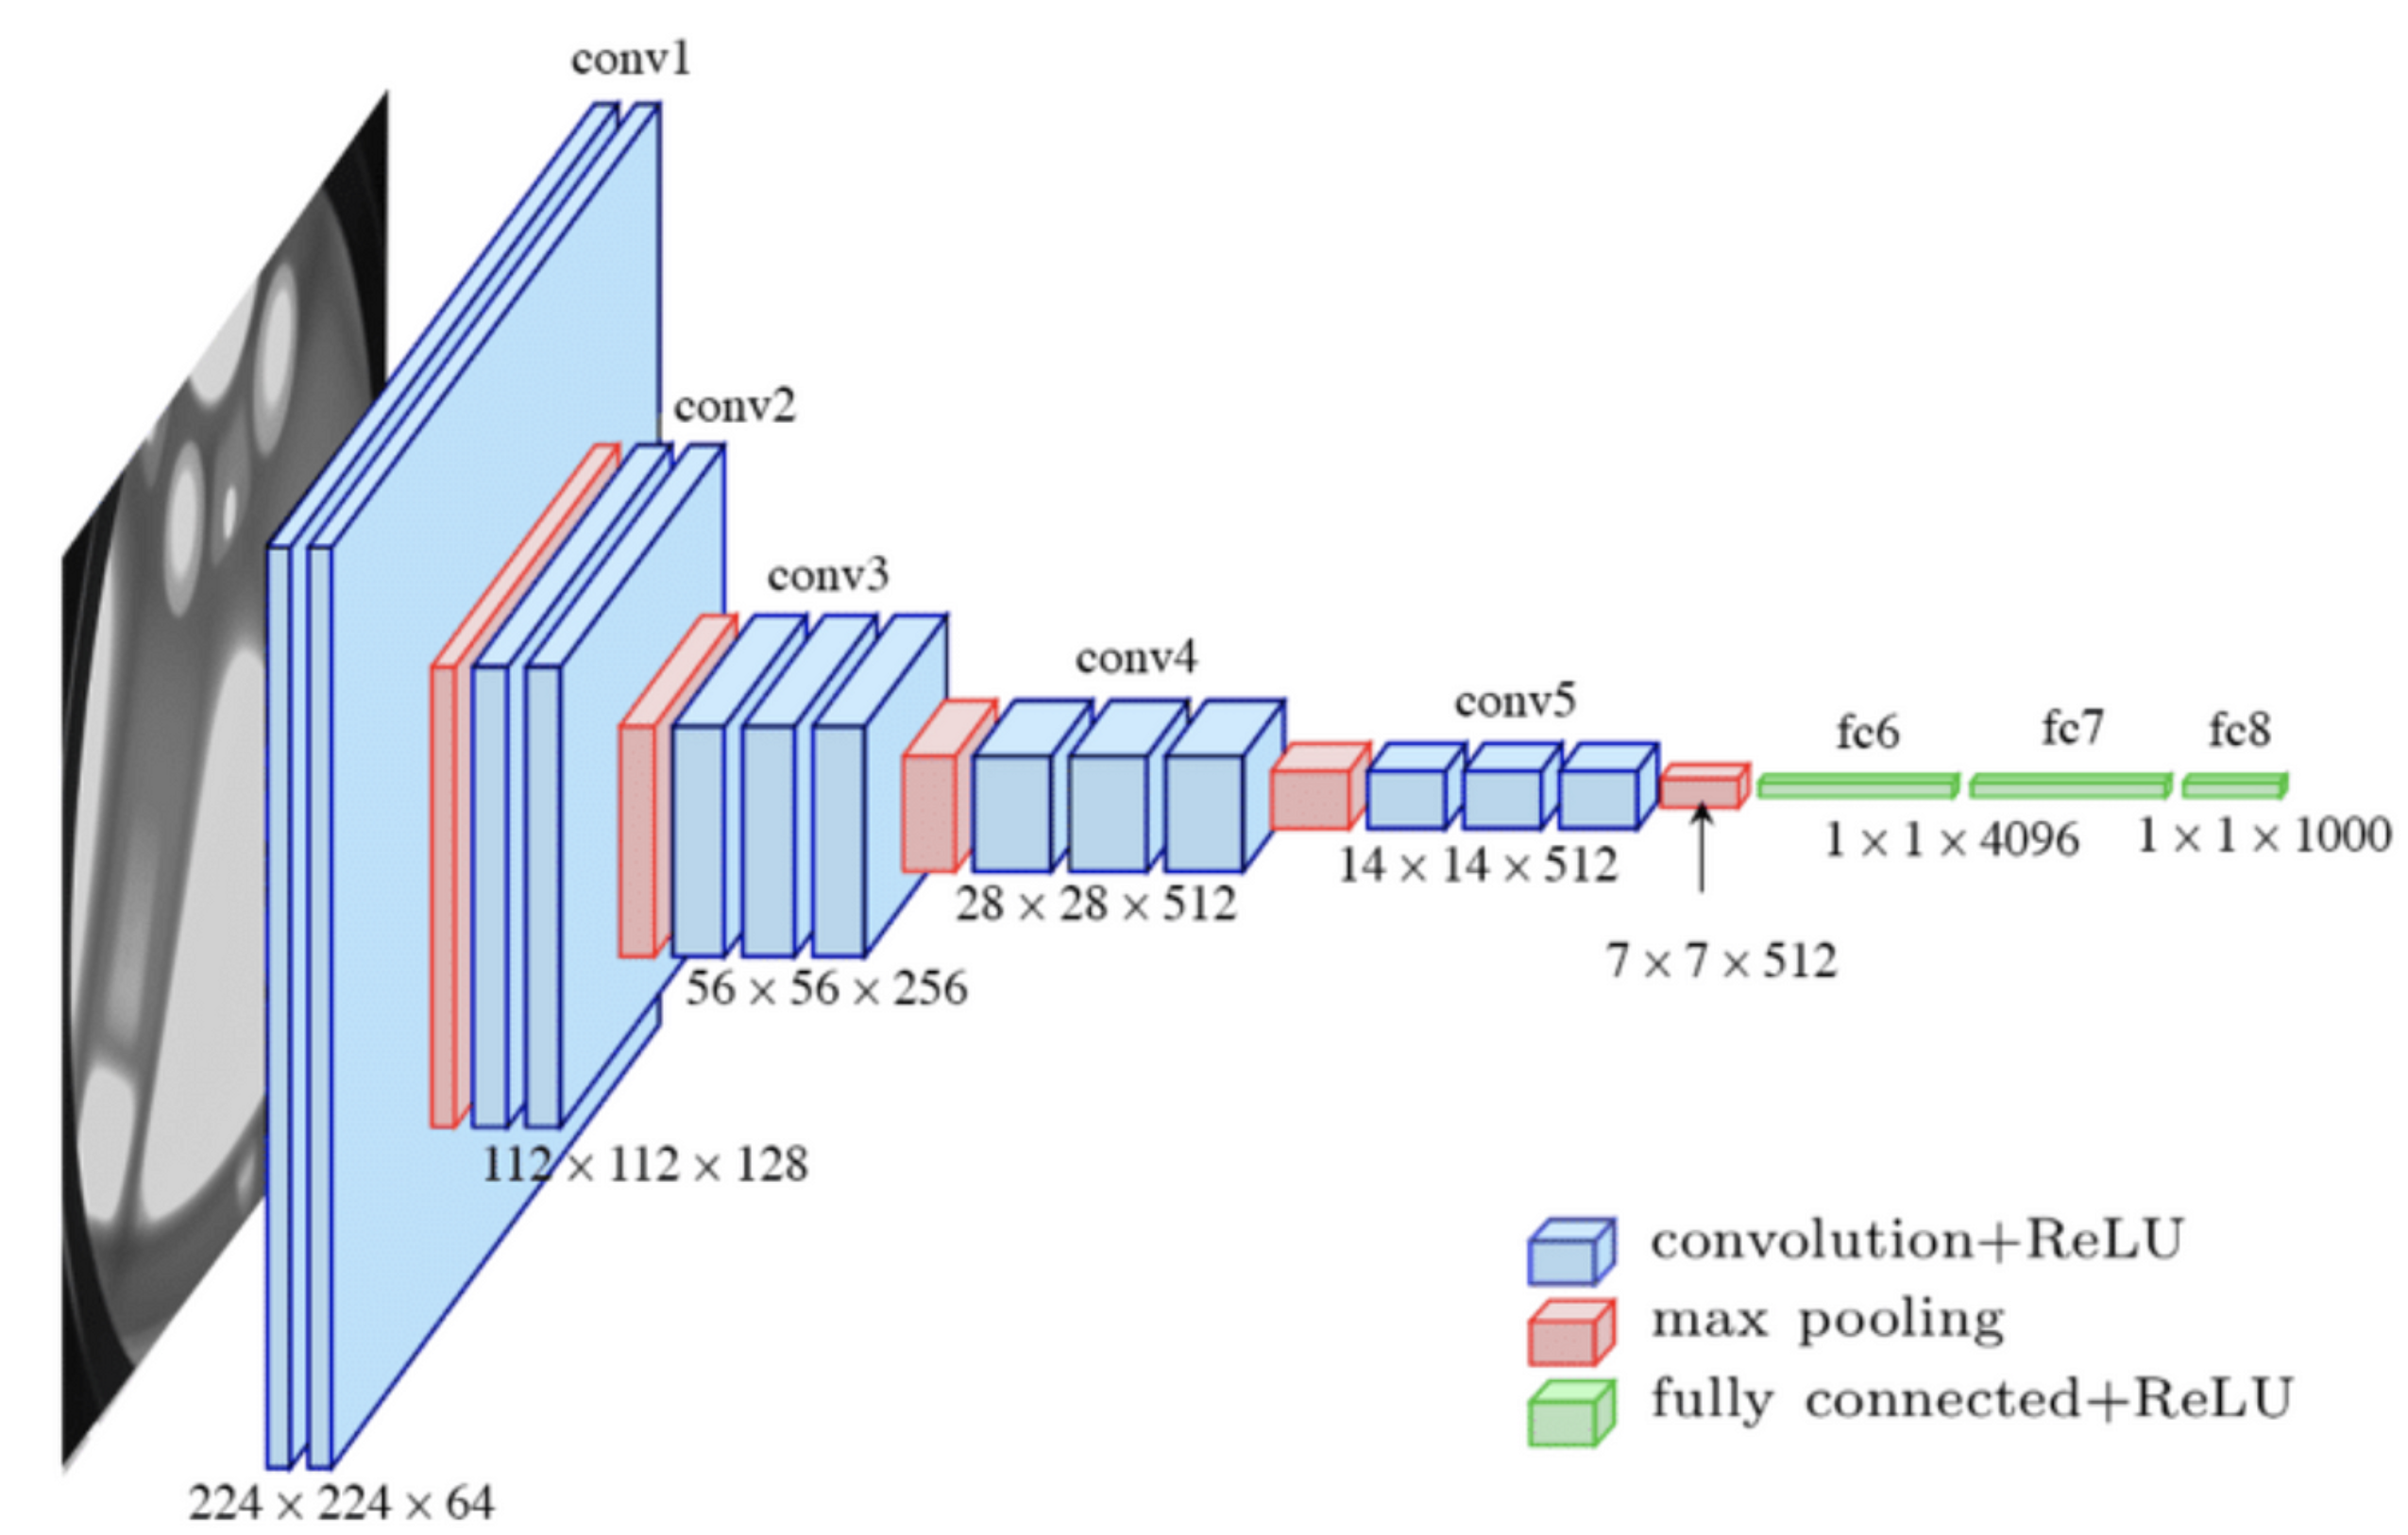
\includegraphics[height=6cm]{images/jcnn/vgg16.png}
  \caption{Graphic representation of the VGG-16 architecture, presenting the different kind of layer composing the architecture.}
  \label{fig:jcnn:vgg16}
\end{figure}

\subsection{Model}
\label{sec:jcnn:model}

The architecture we use is derived from the VGG-16 architecture \cite{simonyan_very_2015} illustrated in figure \ref{fig:jcnn:vgg16}. We define a set of hyperparameters which values are presented in table \ref{tab:jcnn:hyper}. $N_{blocks}$ is the number of convolution blocks, a block being composed of two convolutional layers with $3\times3$ filters using ReLU activation function, a $3\times3$ max-pooling layer (except for the last block) and a dropout layer. The number of channels is dependent of the depth of the block $N^i_{channels} = i * N_{channels}, i \in [1..N_{blocks}]$.

The result of the last convolution layer is then flattened then fed forward to the FCDNN. Its configuration is expressed as a sequential of fully connected layer using the PReLU activation function. For example $2 * 1024 + 2 * 512$ is the sequence of 2 layers with a width of 1024 followed by 2 other layers with a width of 512. Finally the last layer is 4 neurons wide without activation function, one for each component of the interaction vertex: Energy, X, Y, Z.

We explore in this work two different activation functions
\begin{align}
  (E+V)(E, x, y, z) &= \bigg\langle (E - E_{true})^2 + 0.85 \sum_{\lambda \in [x, y, z]} (\lambda - \lambda_{true})^2 \bigg\rangle \\
  (E_r + V_r)(E, x, y, z) &=  \bigg\langle \frac{(E - E_{true}) ^ 2}{E_{true}} + \frac{10}{R} \sum_{\lambda \in [x, y, z]} (\lambda - \lambda_{true})^2 \bigg\rangle
\end{align}
where $R$ is the radius of the CD. With the energy in MeV and the distance in meters, we use the factor 0.85 and 10 to equilibrate the two term of the loss function so they have the same magnitude.
\begin{itemize}
  \item The loss function $(E+V)$ is close to a simple Mean Squared Error (MSE). MSE is one of the most basic loss function, the derivative is simple and continuous in every point. It is a strong starting point to explore the possibility of CNNs.
  \item $(E_r + V_r)$ can be see as a relative MSE.
\end{itemize}
The idea is that: due to the inherent statistic uncertainty over the number of collected Number of Photo Electrons (NPE), the absolute resolution $\sigma (E - E_{true})$ will be larger at higher energy than at low energy. But we expect the \textit{relative} energy resolution $\frac{\sigma(E - E_{true})}{E_true}$ to be smaller at high energy than lower energy as illustrated in figure \ref{fig:juno:rec:qtmle}. Because of this, by using simple MSE the most important part in the loss come from the high energy part of the dataset whereas with a relative MSE, the most important become the low energy events in the dataset. We hope that by using a relative MSE, the neural network will focus on low energy events where the reconstruction is considered the hardest part of the dataset.


\begin{table}[ht]
  \centering
  \begin{tabular}{ | c | c | }
    \hline $N_{blocks}$ & {2, 3, 4} \\
    \hline $N_{channels}$ & {32, 64, 128} \\
    \hline
    \multirow{4}{*}{FCDNN configuration} & 2 * 1024 \\
                                        & 2 * 2048 + 2 * 1024 \\
                                        & 3 * 2048 + 3 * 512 \\
                                        & 2 * 4096 \\
    \hline
    Loss & $E+V$, $E_r + V_r$ \\
    \hline
  \end{tabular}
  \caption{Hyperparameters used for the CNN}
  \label{tab:jcnn:hyper}
\end{table}

Each one of the combination of those hyperparameters is then tested and compared to each other over an analysis sample. We cannot use the mean loss because we consider multiple loss function so we use multiple observables:
\begin{itemize}
  \item The mean absolute energy error $\langle E \rangle = \langle | E - E_{true} | \rangle$. It is an indicator of the energy bias of our reconstruction.
  \item The standard deviation of the energy error $\sigma E = \sigma (E - E_{true})$. This the indicator on our precision in energy reconstruction.
  \item The mean distance between the reconstructed vertex and the true vertex $\langle V \rangle = \langle | \vec{V} - \vec{V}_{true} | \rangle$. This an indicator of the bias and precision of our vertex reconstruction.
  \item The standard deviation of the distance between the true and reconstructed vertex $\sigma V = \sigma |\vec{V} - \vec{V}_{true}|$. This is an indicator if the precision in our vertex reconstruction.
\end{itemize}

For the vertex indicator, it is worth noting that $\langle V \rangle$ is not expected to be zero and so if unfit to be used for the loss. Indeed, let's say we consider error on each of the component as random variable following a normal distribution. We allow ourself to use this representation as our signal possess a strong statistical uncertainty in NPE that follow a Poisson law, i.e. a Gaussian law $\mathcal{N}$ when NPE is high enough which is the case for our signal. So following:
\begin{equation}
  \Delta V = |\vec{V} - \vec{V}_{true}| = \sqrt{\Delta X^2 + \Delta Y^2 + \Delta Z^2}; ~ \Delta X, \Delta Y, \Delta Z \sim \mathcal{N}
\end{equation}
then
\begin{equation}
  \Delta V \sim \chi
\end{equation}
where $\chi$ is a Chi law which probability density function is different from 0 only in $\mathbb{R}^+$

\subsection{Data representation}
\label{sec:jcnn:data}
\begin{itemize}
  \item Data is 240x240 images
    \begin{itemize}
      \item Following $\theta$ and $\phi$ distribution, explain the coordinate system of JUNO
      \item Optimized for $\approx$ 1 SPMT/pixel
      \item 1 Charge channel
      \item 1 Time channel
    \end{itemize}
  \item Discuss data format
    \begin{itemize}
      \item Empty pixel ? -> $Q = 0$, $T = 0$, what does it means/says ? 0 = no signal in a way
      \item Image distortion
        \begin{itemize}
          \item \textbf{Maybe speak of this in the conclusion ?} Could be done in two step:
          \item 1. Reconstruct $\theta$ and $\phi$
          \item 2. "Rotate" the image so the event is at the center of the image -> Prevent distortion + reconstruction E and R become pseudo rotational invariant (as they should be)
        \end{itemize}
      \item 1 Millions MC e+ events for training (900k for train, 50k for validation and 50k for test)
        \begin{itemize}
          \item MC for the moment, will need to retrain with mix of calibration data (Good question, is the CNN PID agnostic ?)
          \item 47 IBD/day -> 1M event is 21k days of data (for reference, 6 years of data is 94k events)
          \item Events are "optimistic"
            \begin{itemize}
              \item No pile-up
              \item w/o neutrons
              \item time window is decided by electronics
              \item We want to reconstruct the E from $\bar{\nu_e}$
              \item Difference between multiple E -> $E_{vis}$, $E_{rec}$, $E_k$
            \end{itemize}
        \end{itemize}
    \end{itemize}
\end{itemize}

The data used during this analysis is monte carlo data using the official JUNO simulation software (see section \ref{sec:juno:software} for details). The simulated data is composed of positron events, uniformly distributed in the CD volume and in kinetic energy over $E_k \in [0; 9]$ MeV producing a deposited energy $E_{dep} \in [1.022; 10.022]$ MeV. This is done to mimic the signal produced by the IBD prompt signal. Uniform distribution are used so that the CNN does not learn a potential energy distribution, favoring some part of the energy spectrum instead of other.

This data is represented as $240 \times 240$ images, equivalent to third order tensor, with a charge $Q$ channel and a time $t$ channel. The SPMTs are then projected on the plane following illustrated in figure \ref{fig:jcnn:pmt_rep}, the $x$ position is proportional to $theta$ and the $y$ position is defined by $\phi \sin{\theta}$ in spherical coordinates. $\theta = 0$ is defined as being the top of the detector and $phi = 0$ is defined as an arbitrary direction in the detector. In practice, this is the $phi = 0$ given by the MC simulation.

When two SPMTs are in the same pixel, the charges are summed and the lowest of the hit-time is chosen. This choice come from the fact that we expect the photon propagation to be uniform, there should no physical meaning in two signal photons coming one after the other except that the two PMT are at different position. The SPMTs being located close to each other, the reduction of information into the first hit time should not impact to much the reconstruction, at least less than the intrinsic time resolution and statistic uncertainty. The only potential problem in using this first time come from the Dark Noise (DN). Its time distribution is uniform over the signal and could come before a signal hit on the other SPMT in the pixel. In that case, the time information in the pixel become irrelevant and we lose the time information for this part of the detector.
As illustrated in figure \ref{fig:jcnn:pmt_rep} the dimension have been chosen optimized so that at most two SPMTs are in the same pixel while keeping the number of empty pixels relatively low to prevent this kind of issue.

While it could be possible to use bigger images to prevent overlapping, keeping image small images gives multiple advantages:
\begin{itemize}
  \item As presented in section \ref{sec:jcnn:model}, the convolution filter we use are $3 \times 3$ convolution filter, meaning that if SPMTs would be separated by more that one pixel, the first filter would only see one SPMT per filter. This behavior would be kind of counterproductive as the first convolution block would basically be a transmission layer and would just induce noise in the data.
  \item It keep the network relatively small, while this do not impact the convolution layers, the flatten operation just before the FCDNN make the number parameters in the first layer of it dependent on the size of the image.
  \item It reduce the number of empty pixel in the image.
\end{itemize}
The question of empty pixel is an important question in this data representation. Their is two kind of empty pixel in the data.

\begin{figure}[ht]
  \centering
  \begin{subfigure}[b]{0.48\textwidth}
    \centering
    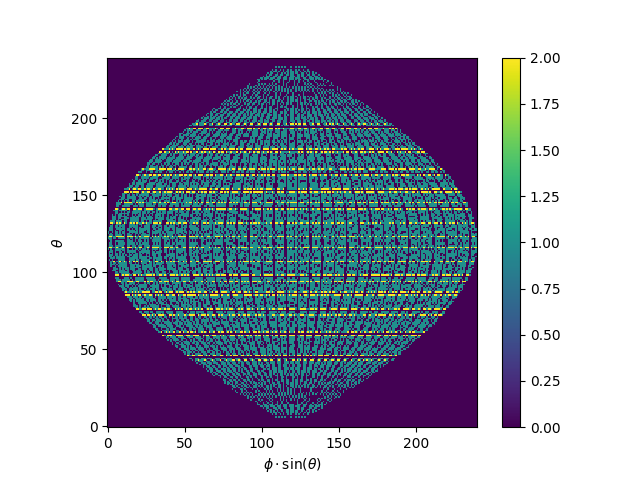
\includegraphics[width=\textwidth]{images/jcnn/pmt_repartition.png}
    \caption{Repartition of SPMTs in the image projection. The color scale is the number of SPMTs per pixel}
    \label{fig:jcnn:pmt_rep}
  \end{subfigure}
  \hfill
  \begin{subfigure}[b]{0.48\textwidth}
    \centering
    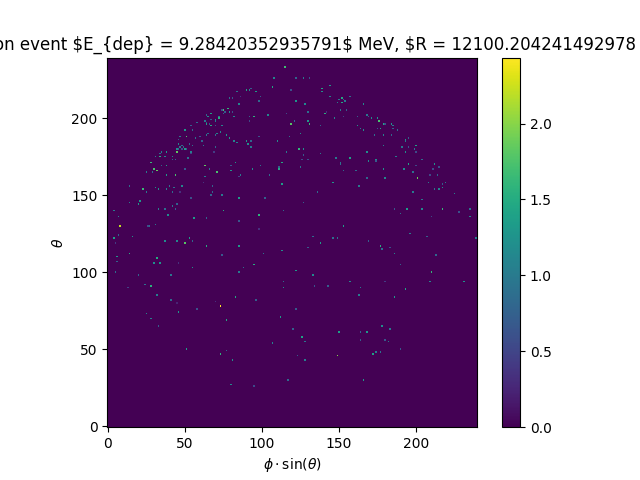
\includegraphics[width=\textwidth]{images/jcnn/illustration_event.png}
    \caption{Example of the charge channel of an event as seen by the CNN \textbf{(Need to redo the title)}}
    \label{fig:jcnn:event_example}
  \end{subfigure}
  \caption{}
\end{figure}

The first kind is pixel that contain a SPMT but the SPMT did not get hit nor registered any dark noise during the event. In this case, the charge layer is zero, which have a physical meaning but then come the question of the time layer. One could argue that the correct time would be infinity (or the largest number our memory allows us) because the hit ``never'' happened, so extremely far from the time of the event. This cause numerical problem as large number, in the linear operation that are happening in the convolution layers, are more signifiant than smaller value. We could try to encode this feature in another way but no number have any significance due to our time being relative to the trigger of the experiment so $-1$ for example is out of question. Float and Double gives us access to special value such as NaN (Not a Number) \cite{noauthor_ieee_2019} but the behavior is to propagate the NaN which leaves us with NaN for energy and position. We choose to keep the value 0 because it's the absorbing element of multiplication and can be though as no activation in the ReLU activation function.

The second kind of pixel is pixel that do not represent parts of the detector such as the corners of the images. The question is basically the same, what to put in the charge and the time channel. The decision is to set the charge and time at 0 following the reasoning presented above. Its important to keep in mind that the fact that a part of the detector that has not been hit is also an information: There is no signal in this part of the detector. This problematic will be explored in more details in chapter \ref{sec:jgnn}.

Another problematic that happens with this representation, and this is not dependent of the chosen projection, is the deformation in the edges of the image and the loss of the neighbouring information in the for the SPMTs at the edge of the image $\phi \sim 180^\circ$. This deformation and neighbouring loss could be partially circumvented as explained in section \ref{sec:jcnn:prospect}
\section{Results}

\begin{itemize}
  \item Comparison with victor results
  \item \textbf{More details when I'll look into the retrained data}
  \item Discuss of the differences
  \item Discuss of the principle of error decorelation
    \begin{itemize}
      \item Possible improvements
      \item Combining algorithms
      \item Average sum
    \end{itemize}
\end{itemize}

\section{Prospect}
\label{sec:jcnn:prospect}

\section{Conclusion}
Intoduction next chapter
